\section{Introduction} \label{intro}
Use \verb|\section| and \verb|\subsection| commands to organize your document. \LaTeX{} handles all the formatting automatically. Use \verb|\label| and \verb|\nameref| commands for cross-referencing sectional headings: the usual \verb|\ref| will not work, as this template uses unnumbered sectional headings. \par
\lipsum[2]

\subsection{Figures and Tables}
Use the table and tabular commands for basic tables --- see \TABLE{example}, for example. For tables, I recommend that you use a separate .tex file for each table and insert it using \verb|\input{mytable.tex}|.

You can upload a figure (JPEG, PNG or PDF) using the project menu. To include it in your document, use the \verb|\includegraphics| command as in the code for \FIG{view}. 

Really wide figures or tables, that take up the entire page, including the gutter space: use \verb|\begin{fullwidth}...\end{fullwidth}| as in \FIG{fullwidth}. And sometimes you may want to use feature boxes like \BOX{simple}.

\begin{figure}
    \begin{fullwidth}
    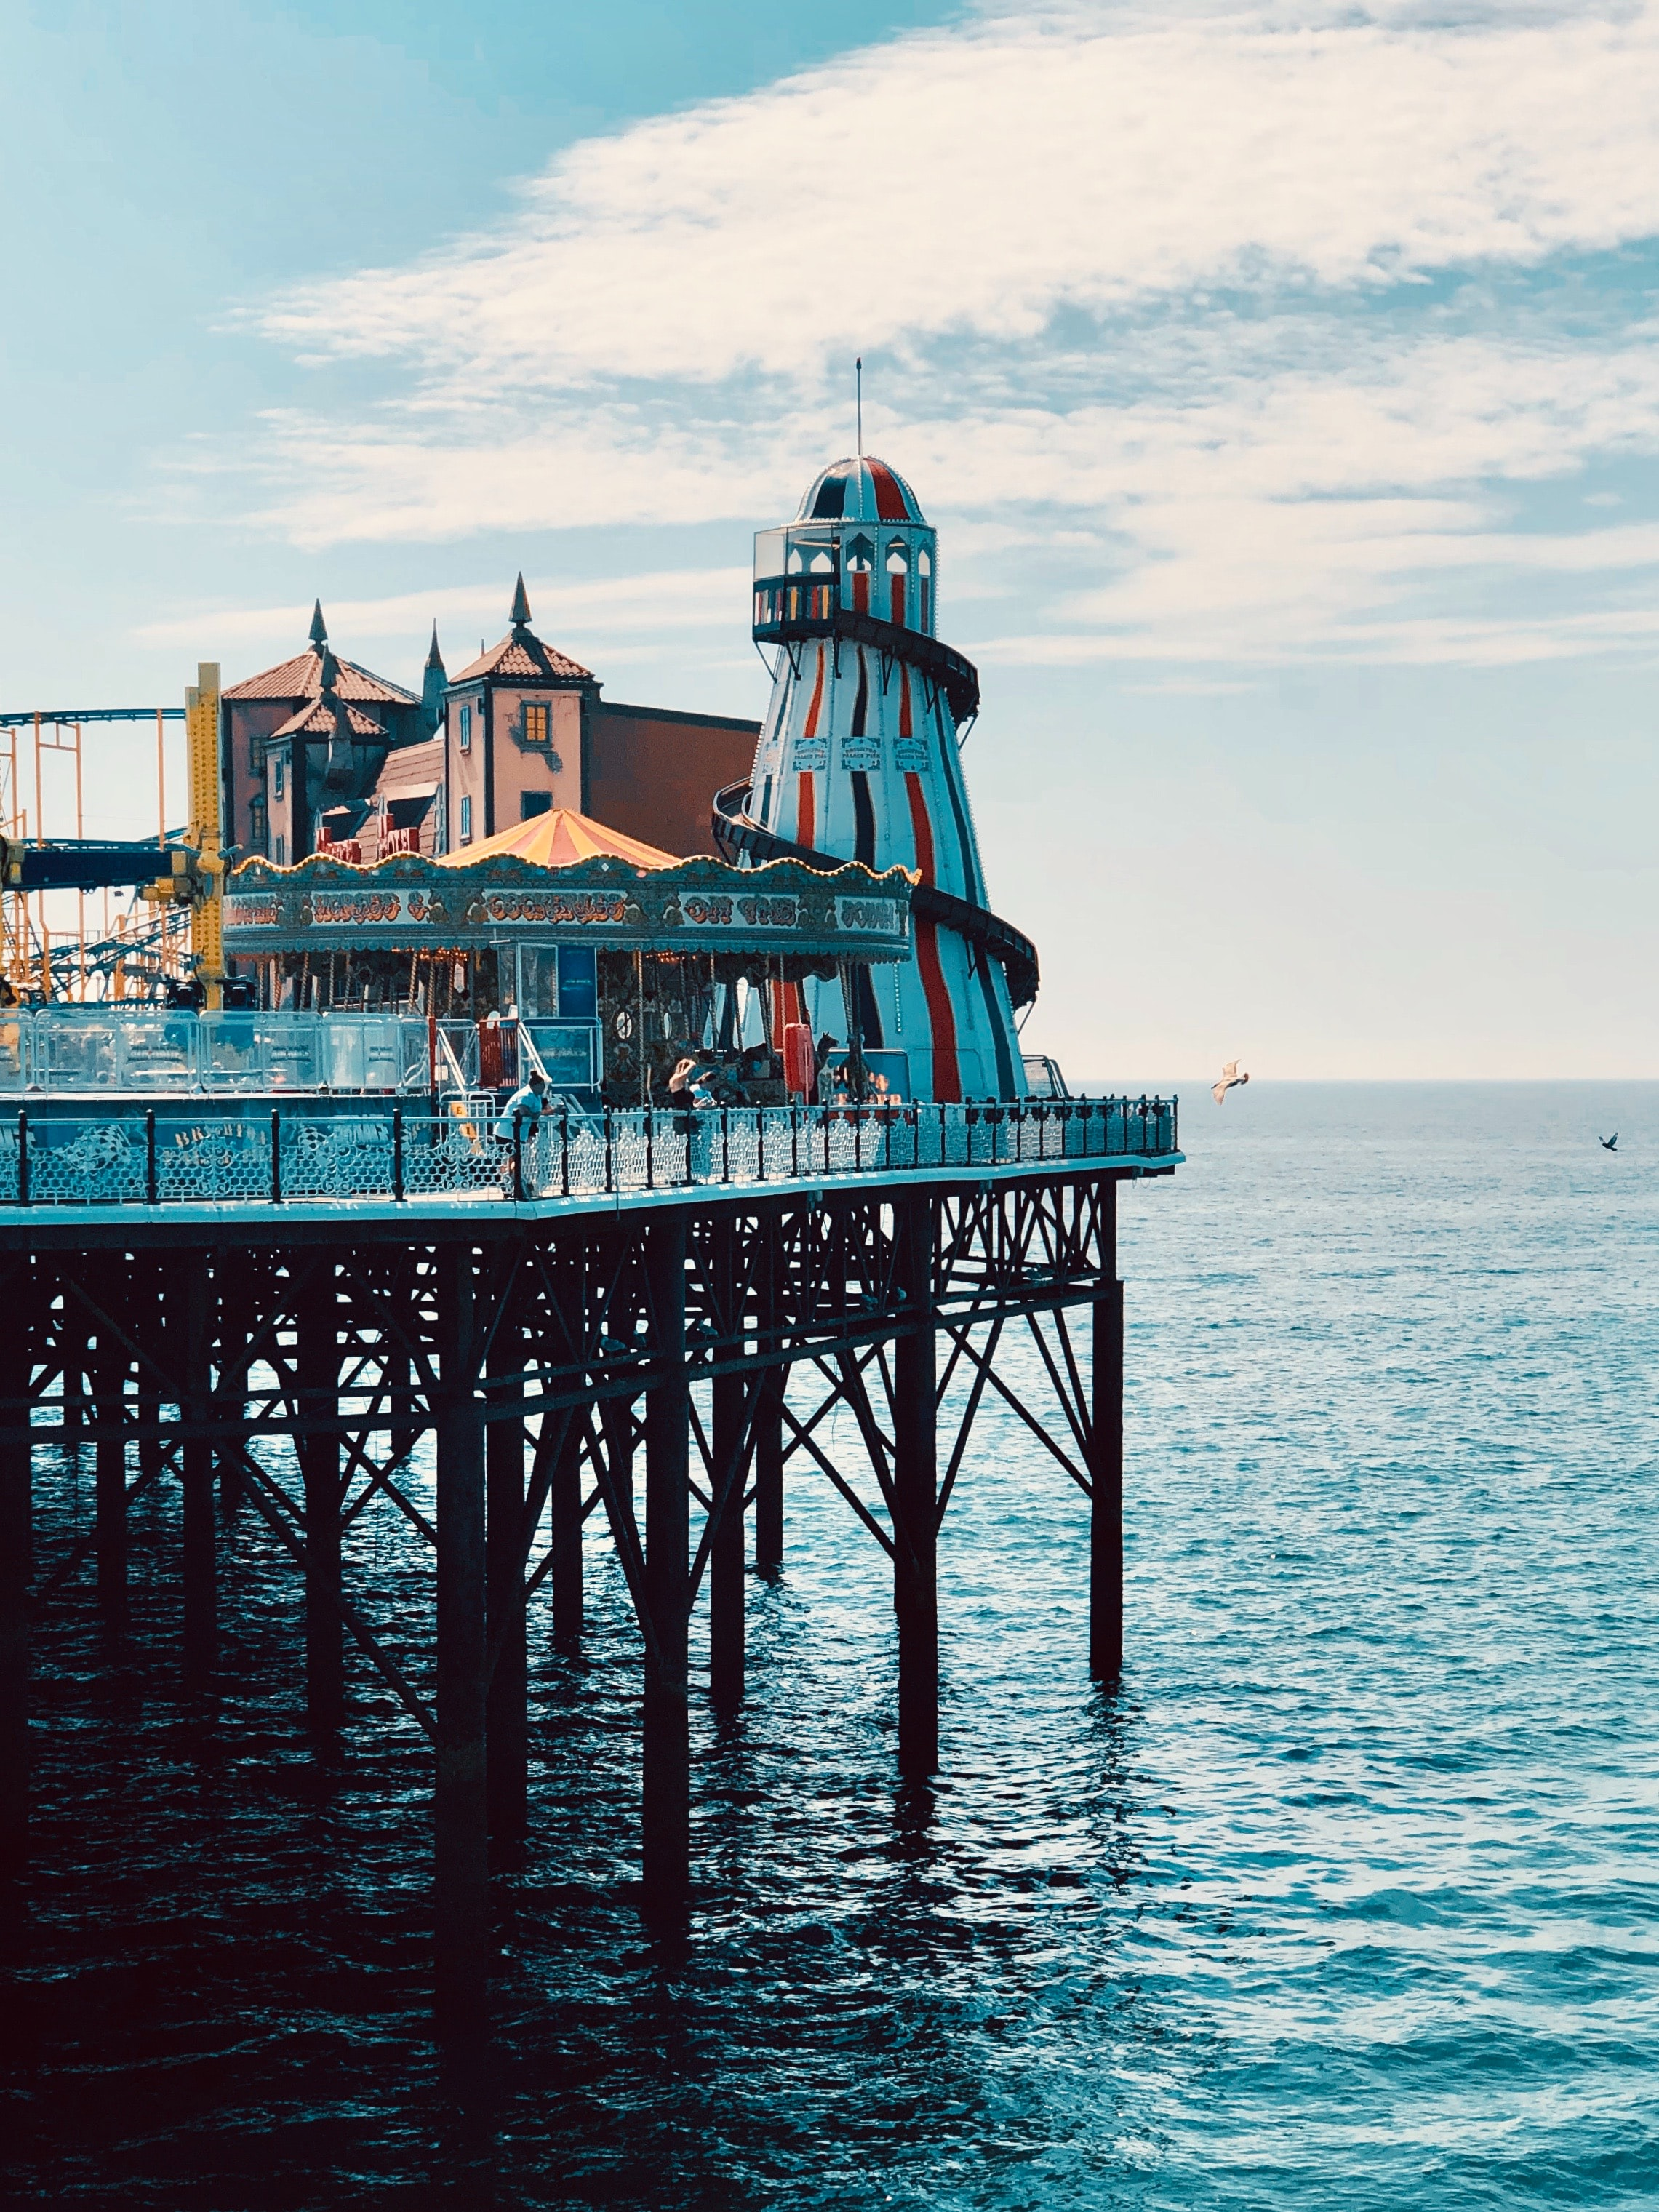
\includegraphics[width=0.65\textheight]{src/figures/brighton.jpeg}
    \caption{\textbf{Photo of lovely Brighton by \href{https://unsplash.com/es/@sanekovs?utm_source=unsplash&utm_medium=referral&utm_content=creditCopyText"}{Alex Ovs} on \href{https://unsplash.com/s/photos/brighton?utm_source=unsplash&utm_medium=referral&utm_content=creditCopyText}{Unsplash}.
    } As a very wide figure that takes up the entire page, including the gutter space.}
    \label{fig:fullwidth}
    \figsupp{There is no limit on the number of Figure Supplements for any one primary figure. Each figure supplement should be clearly labelled, Figure 1--Figure Supplement 1, Figure 1--Figure Supplement 2, Figure 2--Figure Supplement 1 and so on, and have a short title (and optional legend). Figure Supplements should be referred to in the legend of the associated primary figure, and should also be listed at the end of the article text file.}{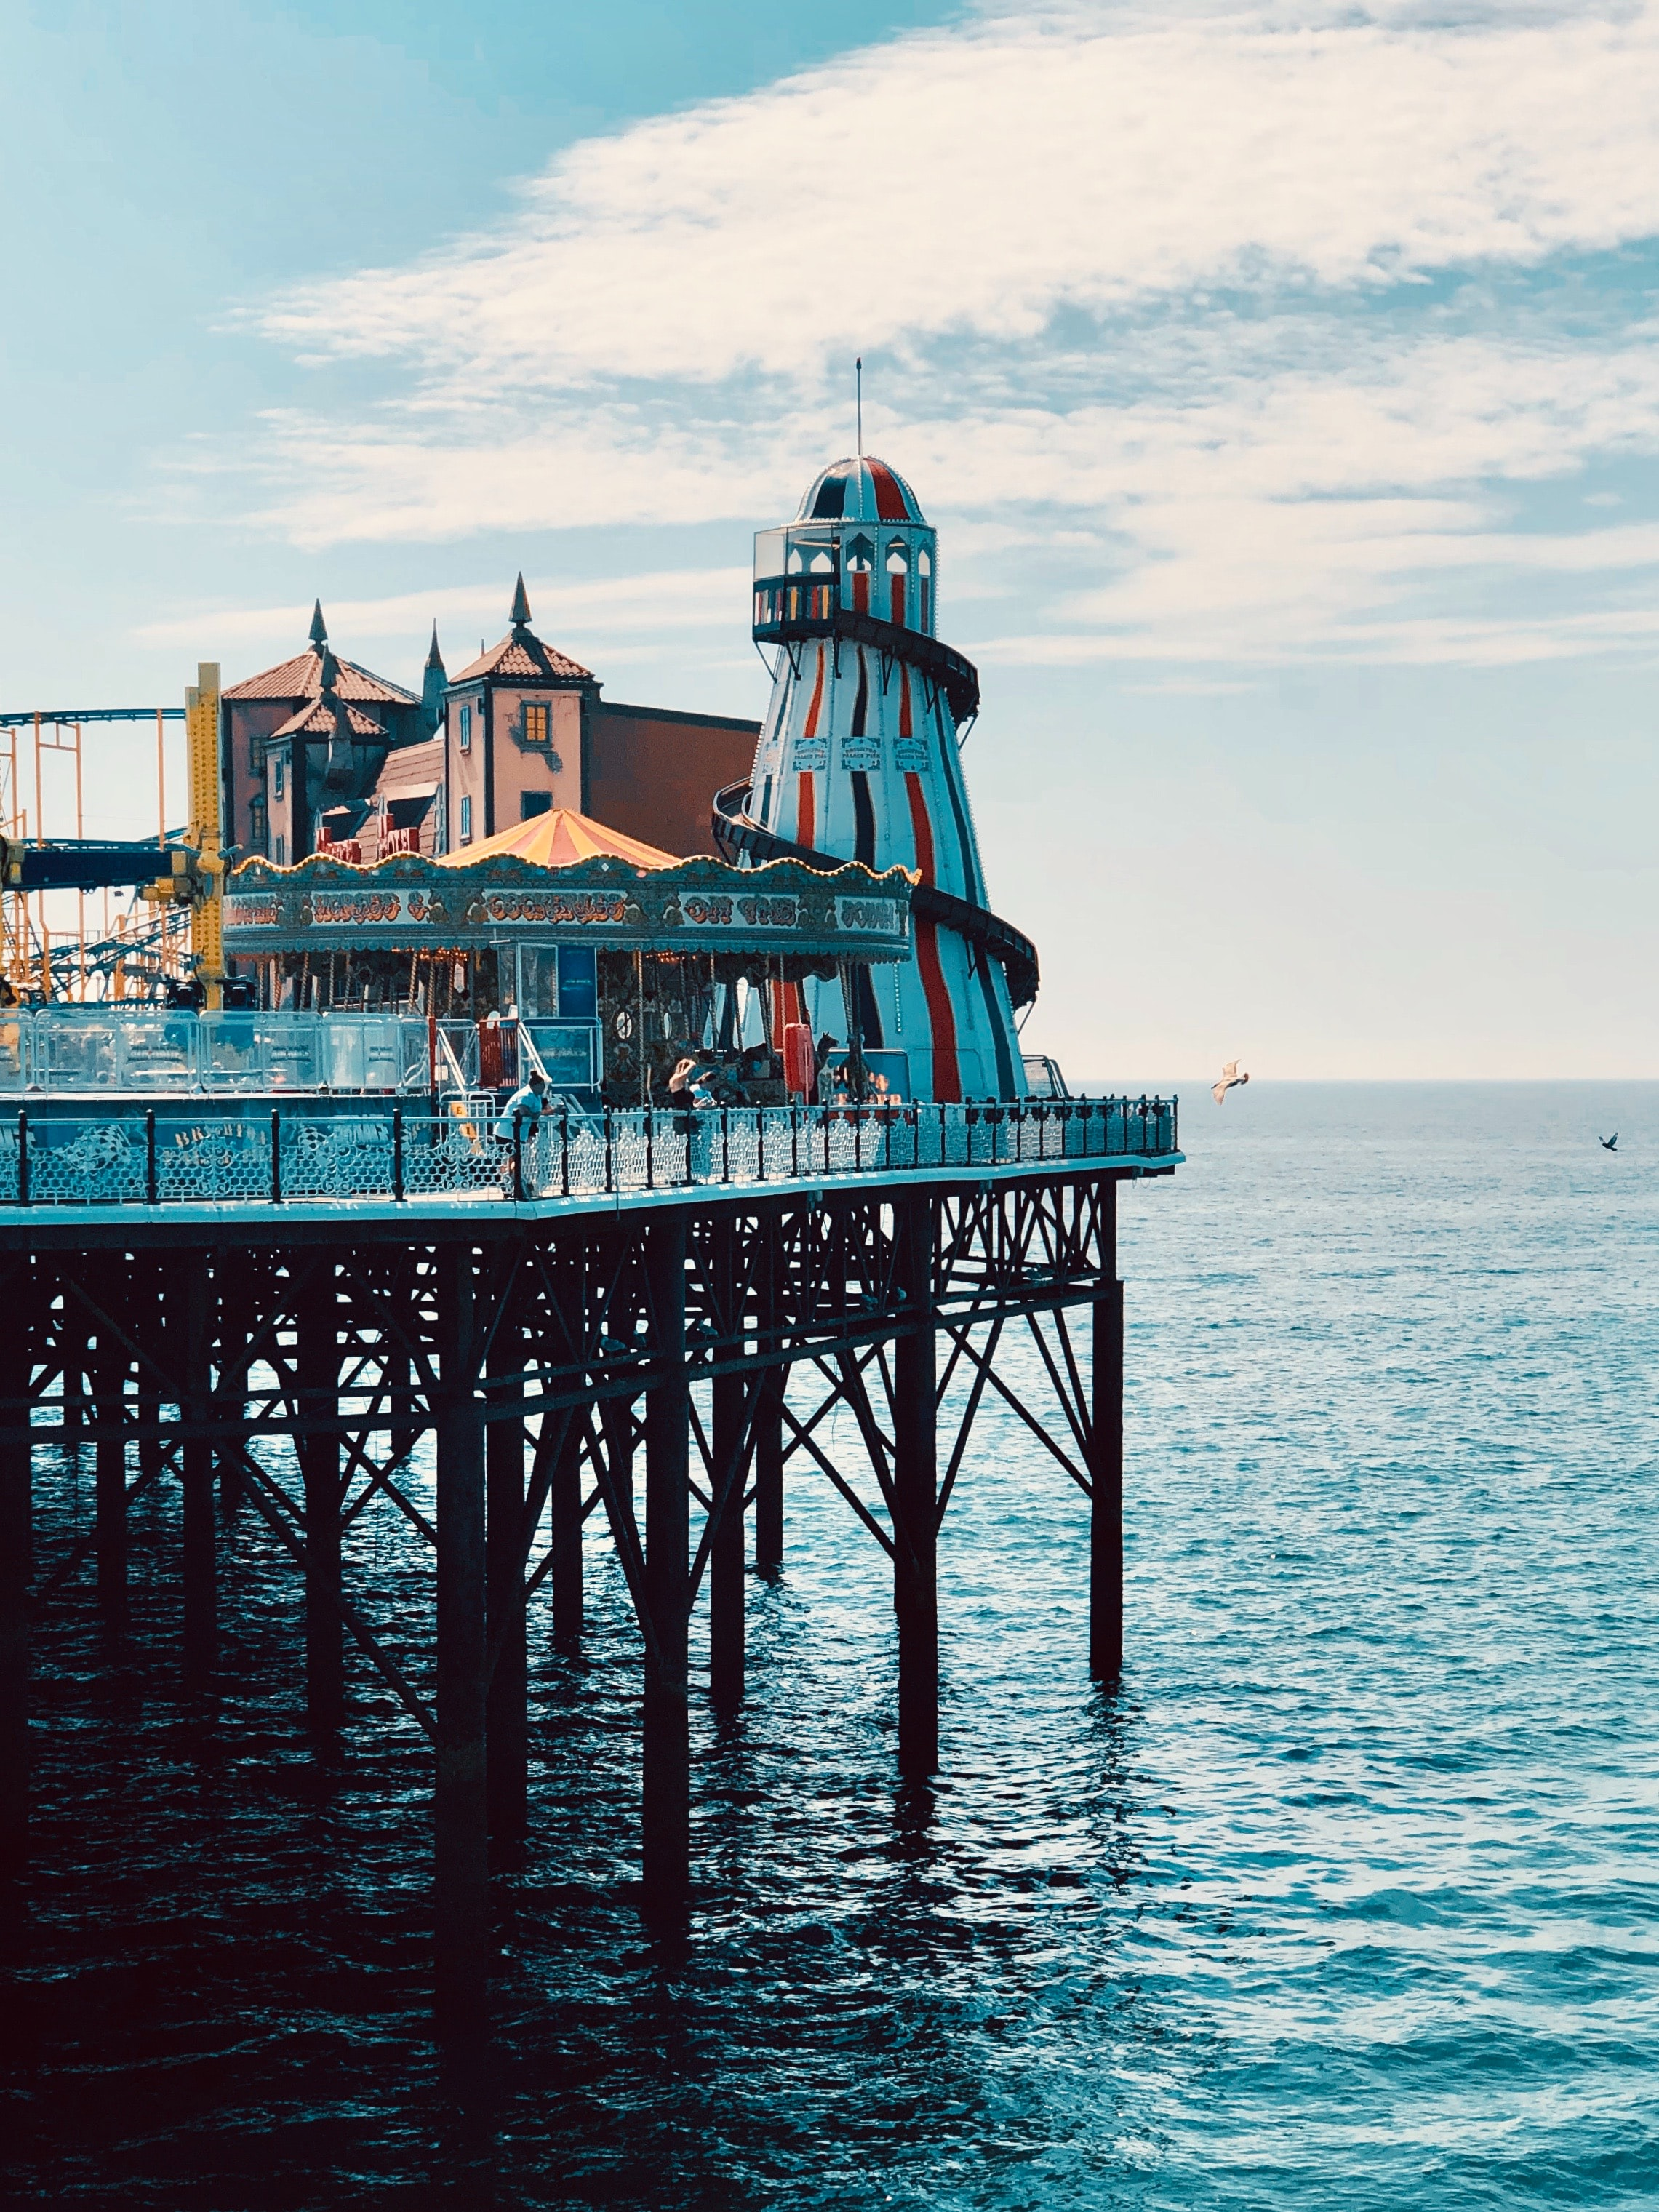
\includegraphics[width=5cm]{src/figures/brighton.jpeg}}
    \end{fullwidth}
\end{figure}

\subsection{Citations and notes}

LaTeX formats citations and references automatically using the bibliography records in your .bib file. Use the \verb|\cite| command for an inline citation, like \cite{Pooley2021}, and the \verb|\parencite| command for a citation in parentheses \parencite{Brembs2021}. Side notes makes good use of the empty margin and can be used ewith the \verb|\sidenote| command. \sidenote{This is a sidenote made with the \textbackslash sidenote package. \lipsum[1]}


\begin{featurebox}
\caption{This is an example feature box}
\label{box:simple}
This is a feature box. It floats!
\medskip

\includegraphics[width=5cm]{example-image}
\featurefig{`Figure' and `table' captions in feature boxes should be entered with \texttt{\textbackslash featurefig} and \texttt{\textbackslash featuretable}. They're not really floats.}

\lipsum[1]
\end{featurebox}

\subsection{Mathematics}

\LaTeX{} is great at typesetting mathematics $abc$. Let $X_1, X_2, \ldots, X_n$ be a sequence of independent and identically distributed random variables with $\text{E}[X_i] = \mu$ and $\text{Var}[X_i] = \sigma^2 < \infty$, and let
\begin{equation}
\label{eq:CLT}
S_n = \frac{X_1 + X_2 + \cdots + X_n}{n}
      = \frac{1}{n}\sum_{i}^{n} X_i
\end{equation}
denote their mean. Then as $n$ approaches infinity, the random variables $\sqrt{n}(S_n - \mu)$ converge in distribution to a normal $\mathcal{N}(0, \sigma^2)$.

You can even get extra fancy and annotate your equations directly: %this uses the `annotate-equations` package. See `https://ctan.org/pkg/annotate-equations` for further info and ideas

\vspace{1.5em} 
\begin{equation}
\label{eq:CLT2}
S_n = \frac{\eqnmarkbox[blue]{a1}{X_1 + X_2 + \cdots + X_n}}{n}
      = \frac{1}{n}\sum_{i}^{n} \eqnmarkbox[purple]{a2}{X_i}
\end{equation}
\annotate[yshift=1em]{above}{a1}{independent and identically distributed random variables}
\annotate[yshift=-1em]{below,left}{a2}{a random variable}
\vspace{1.5em} 

\lipsum[3] 

\begin{figure}
    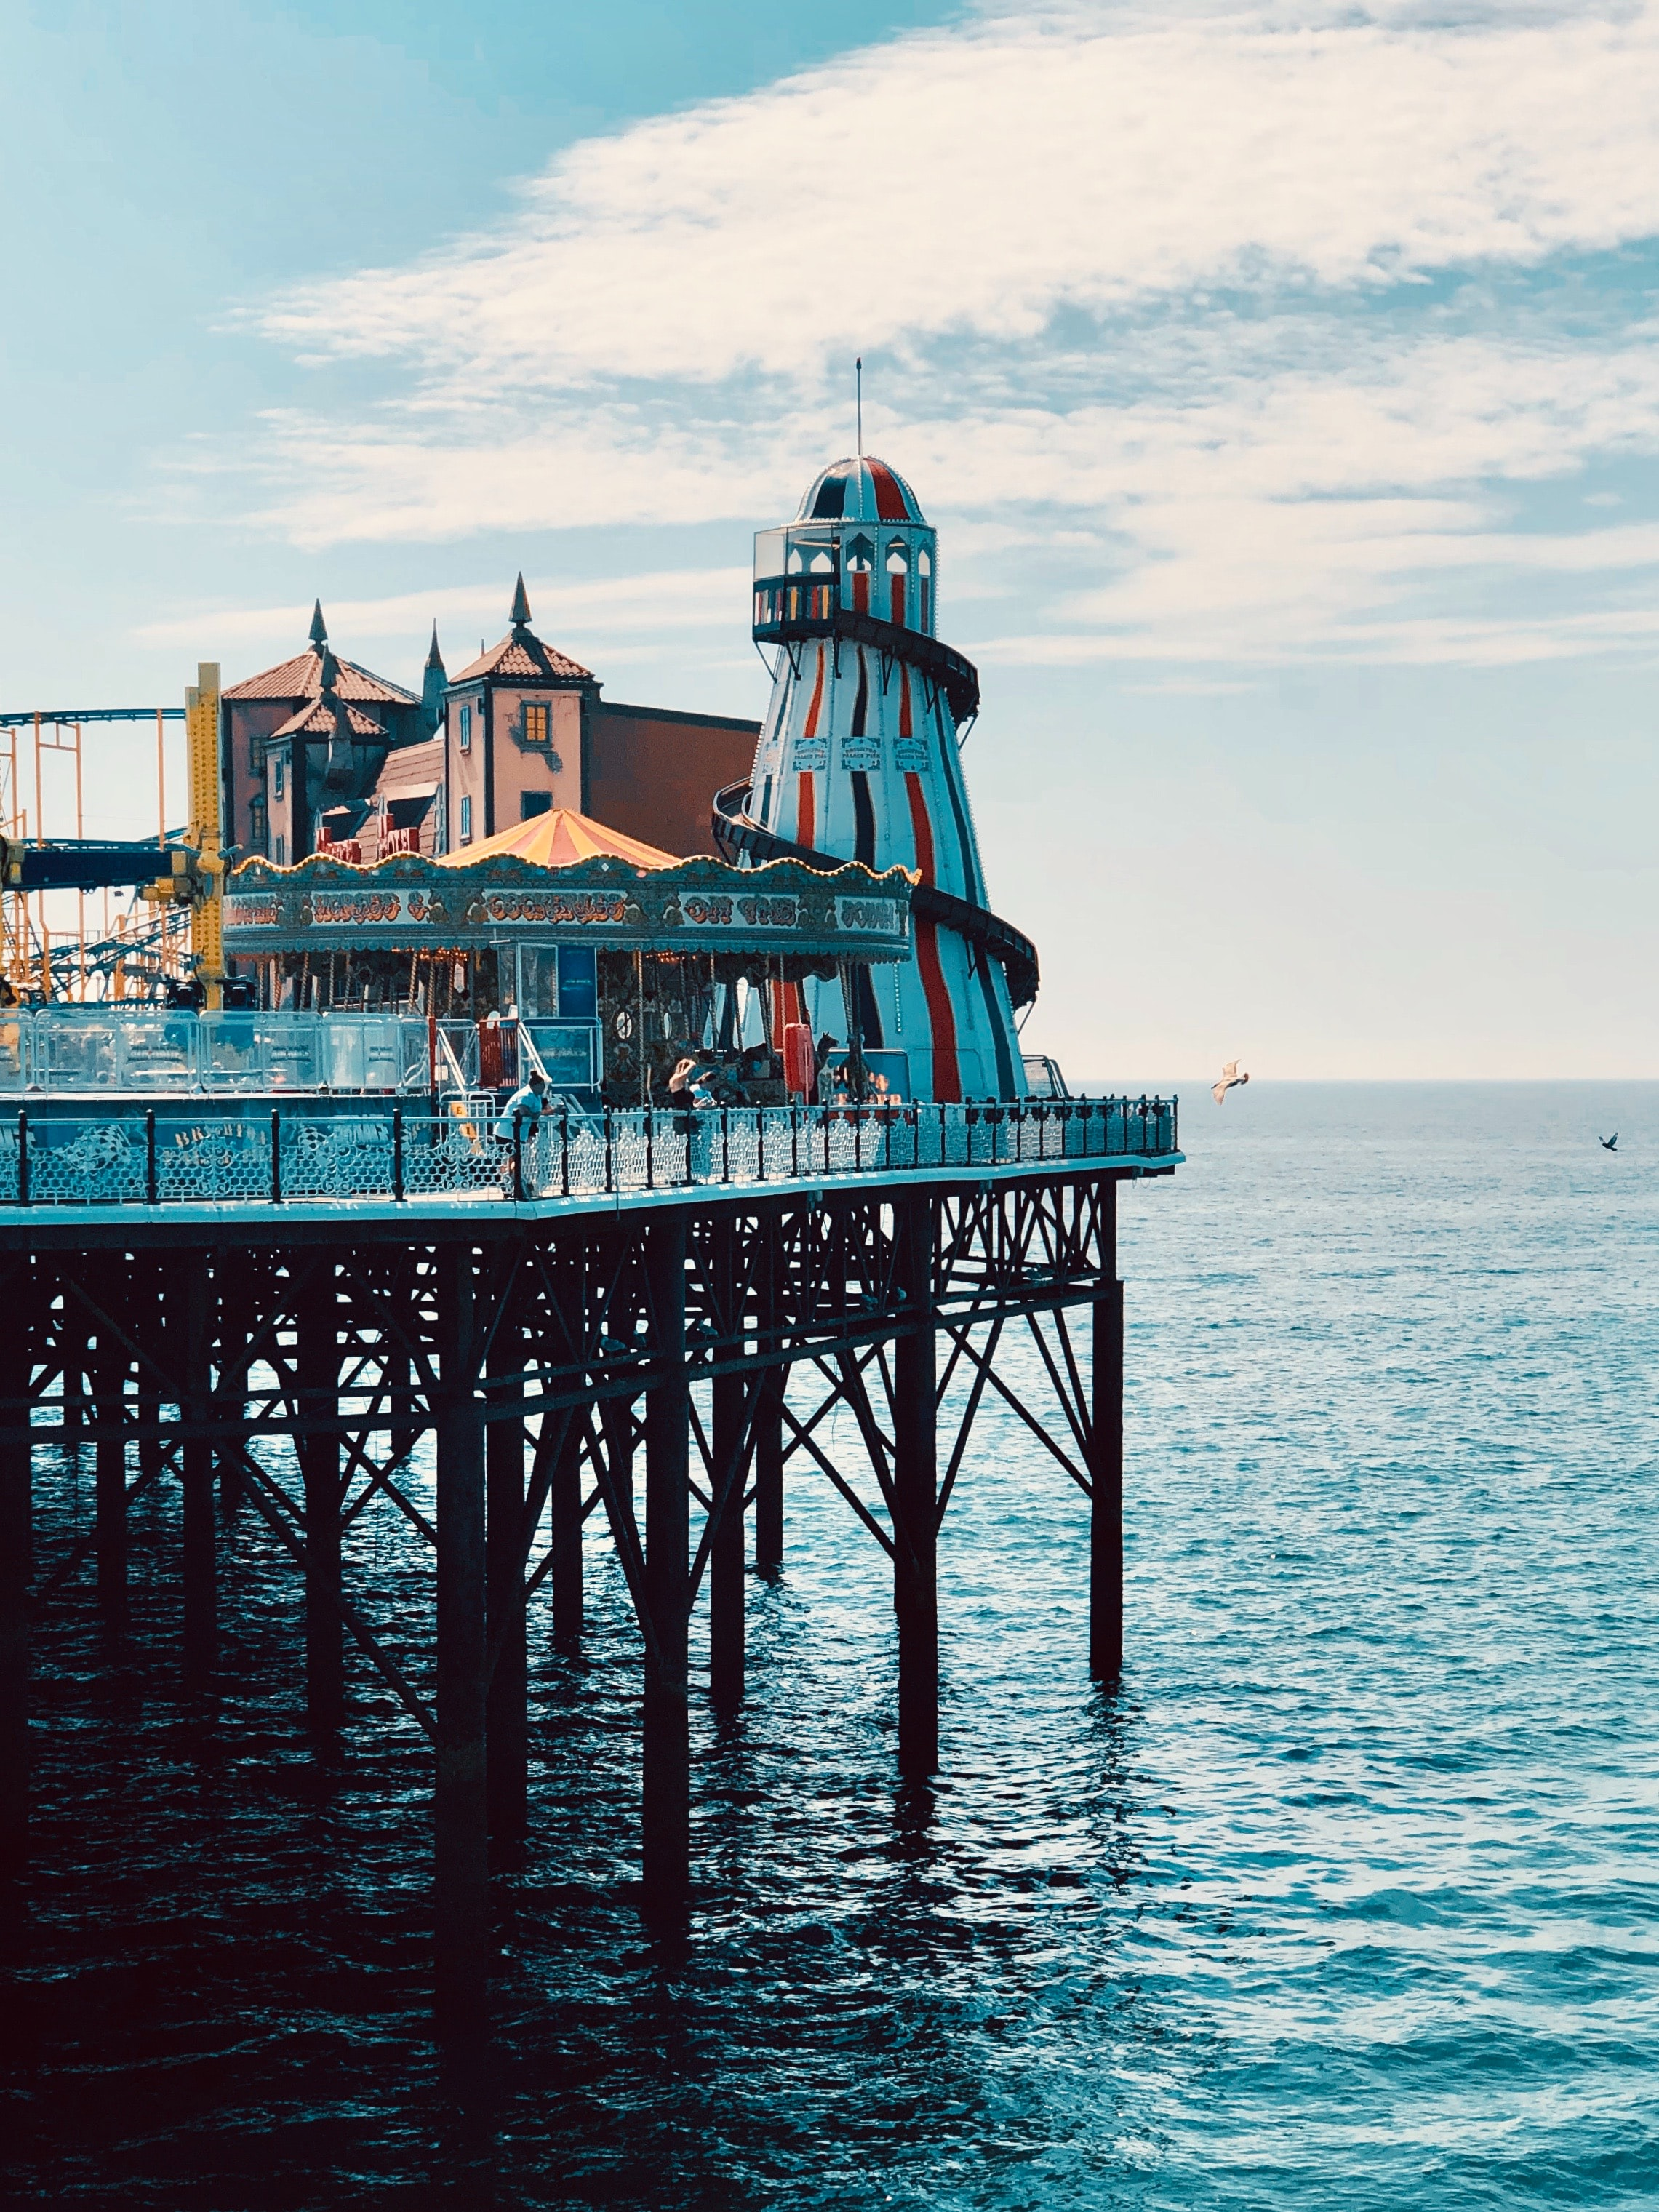
\includegraphics[width=\linewidth]{src/figures/brighton.jpeg}
    \caption{A text-width example.}
    \label{fig:view}
    %% If the optional argument in the square brackets is "none", then the caption *will not appear in the main figure at all* and only the full caption will appear under the supplementary figure at the end of the manuscript.
    \figsupp[Shorter caption for main text.]{This is a supplementary figure's full caption, which will be used at the end of the manuscript.}{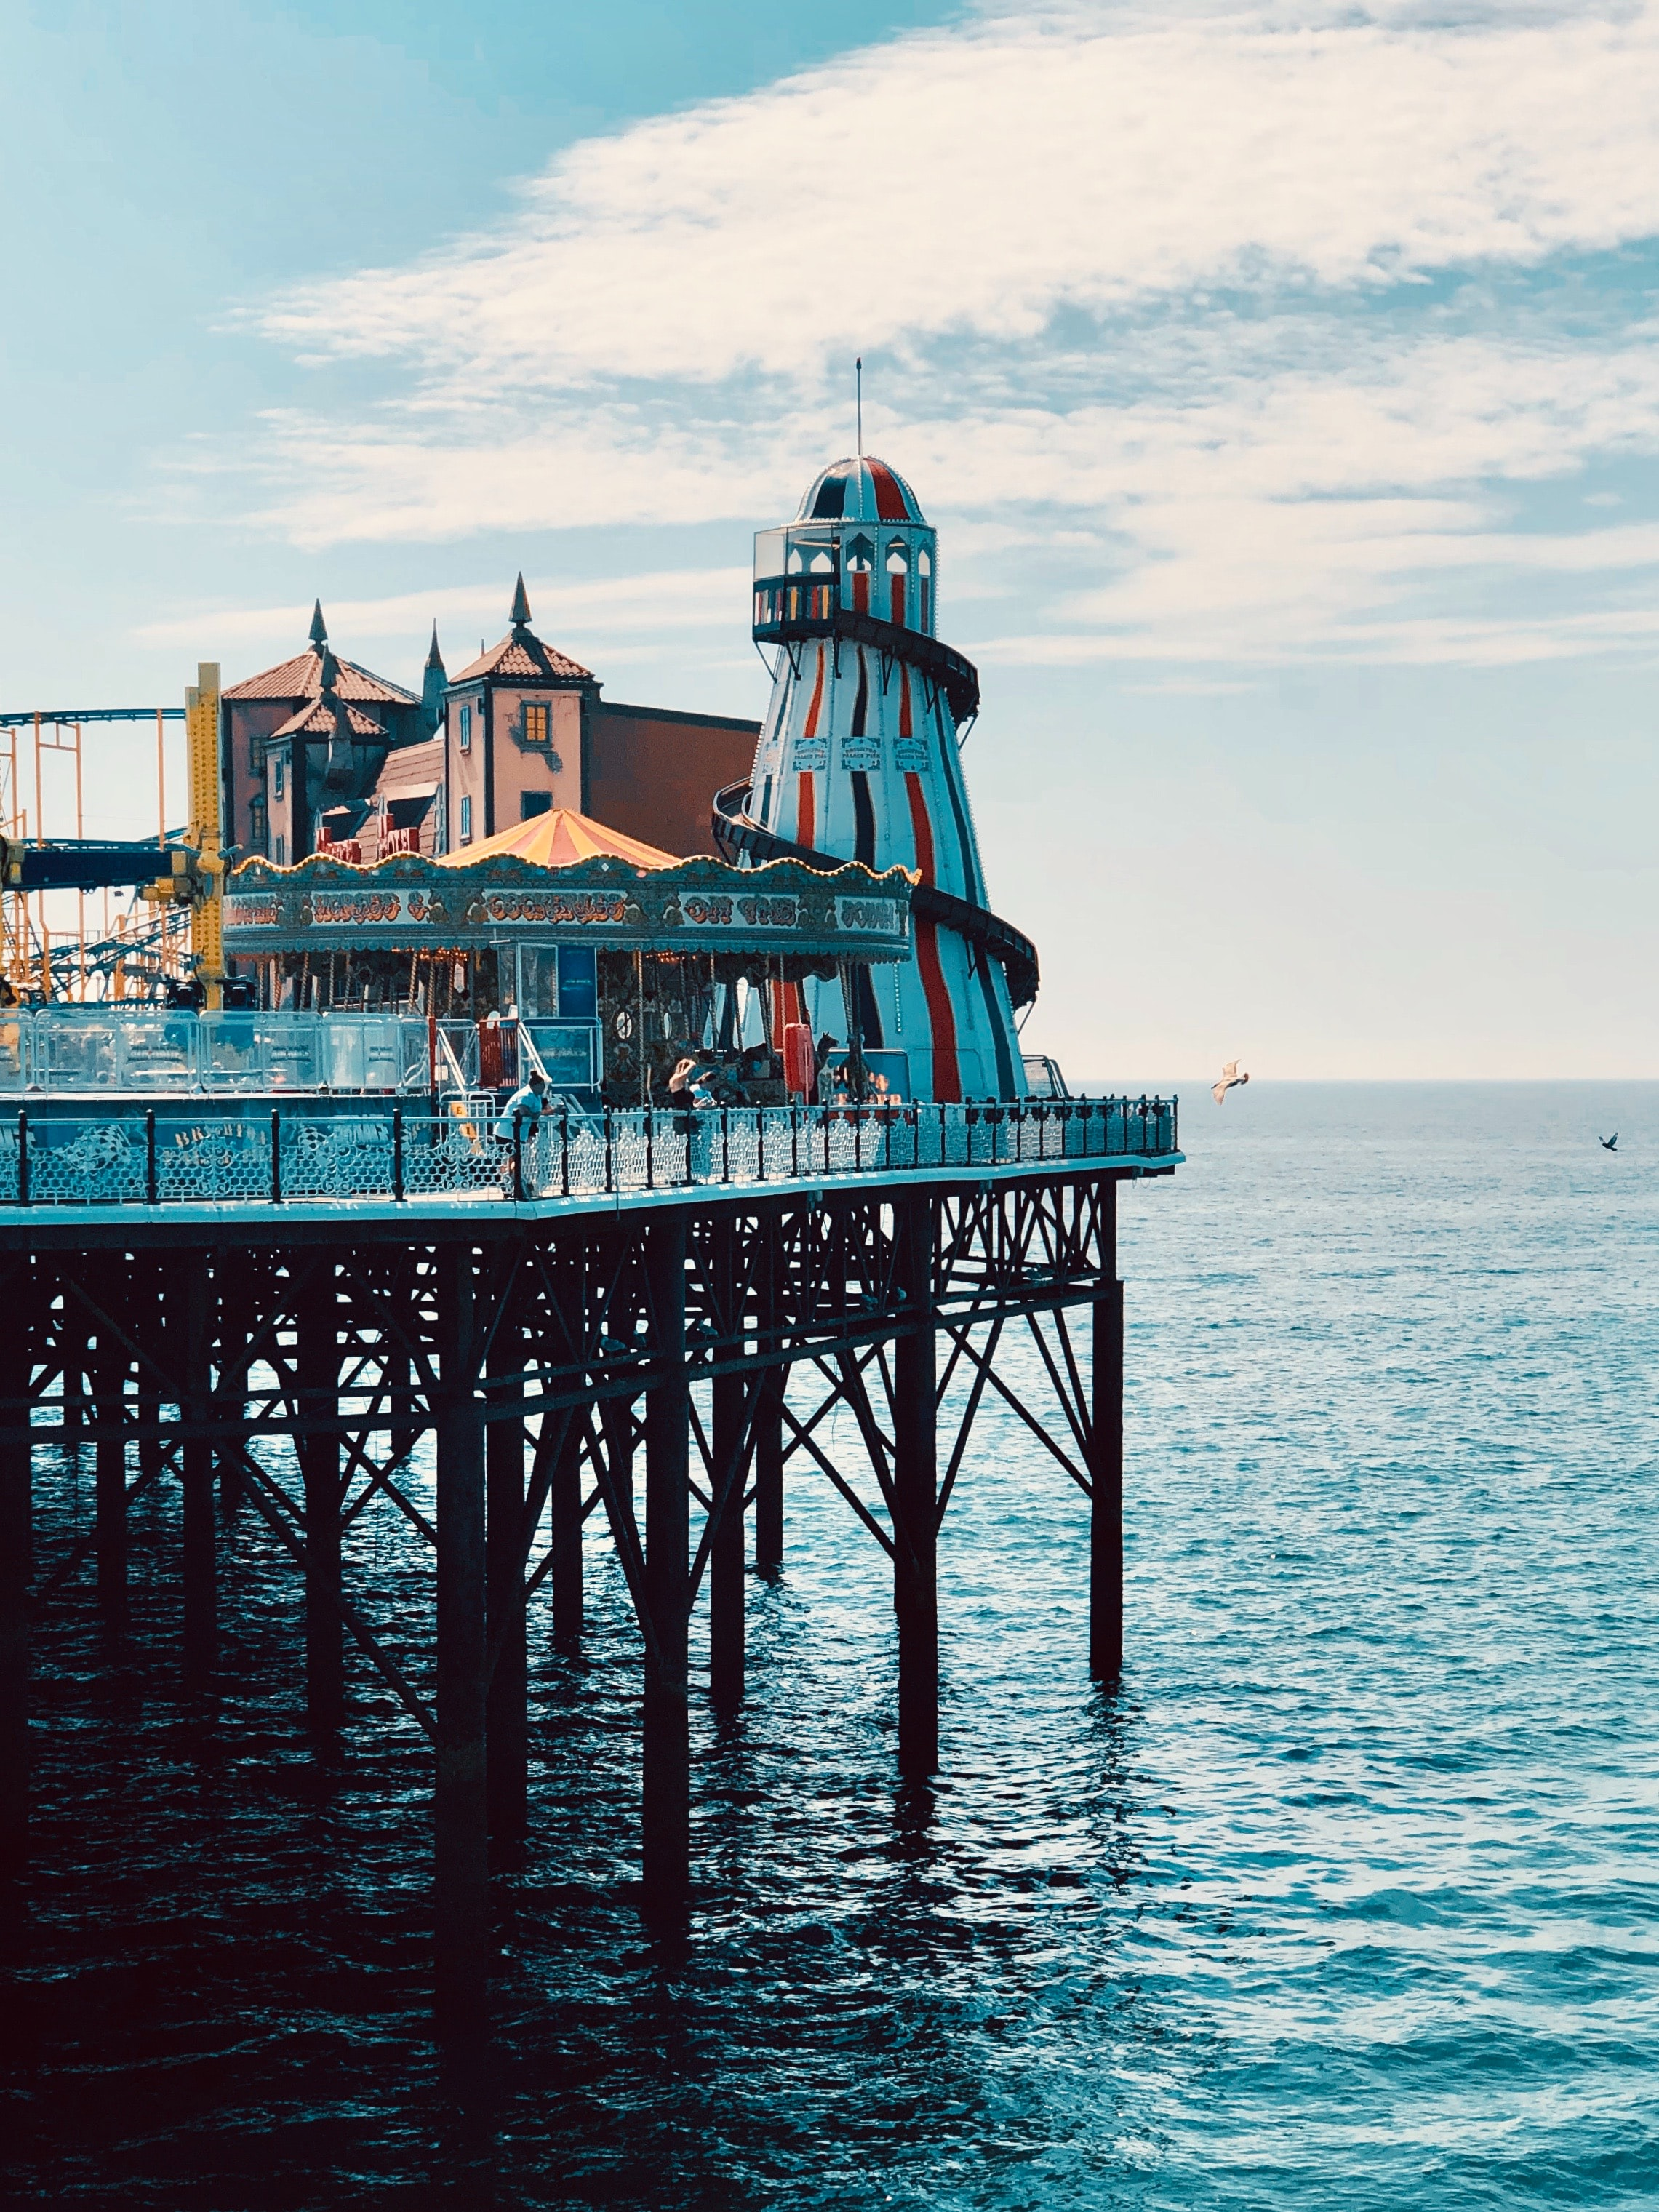
\includegraphics[width=6cm]{src/figures/brighton}}\label{figsupp:sf1}
    \figsupp{This is another supplementary figure.}{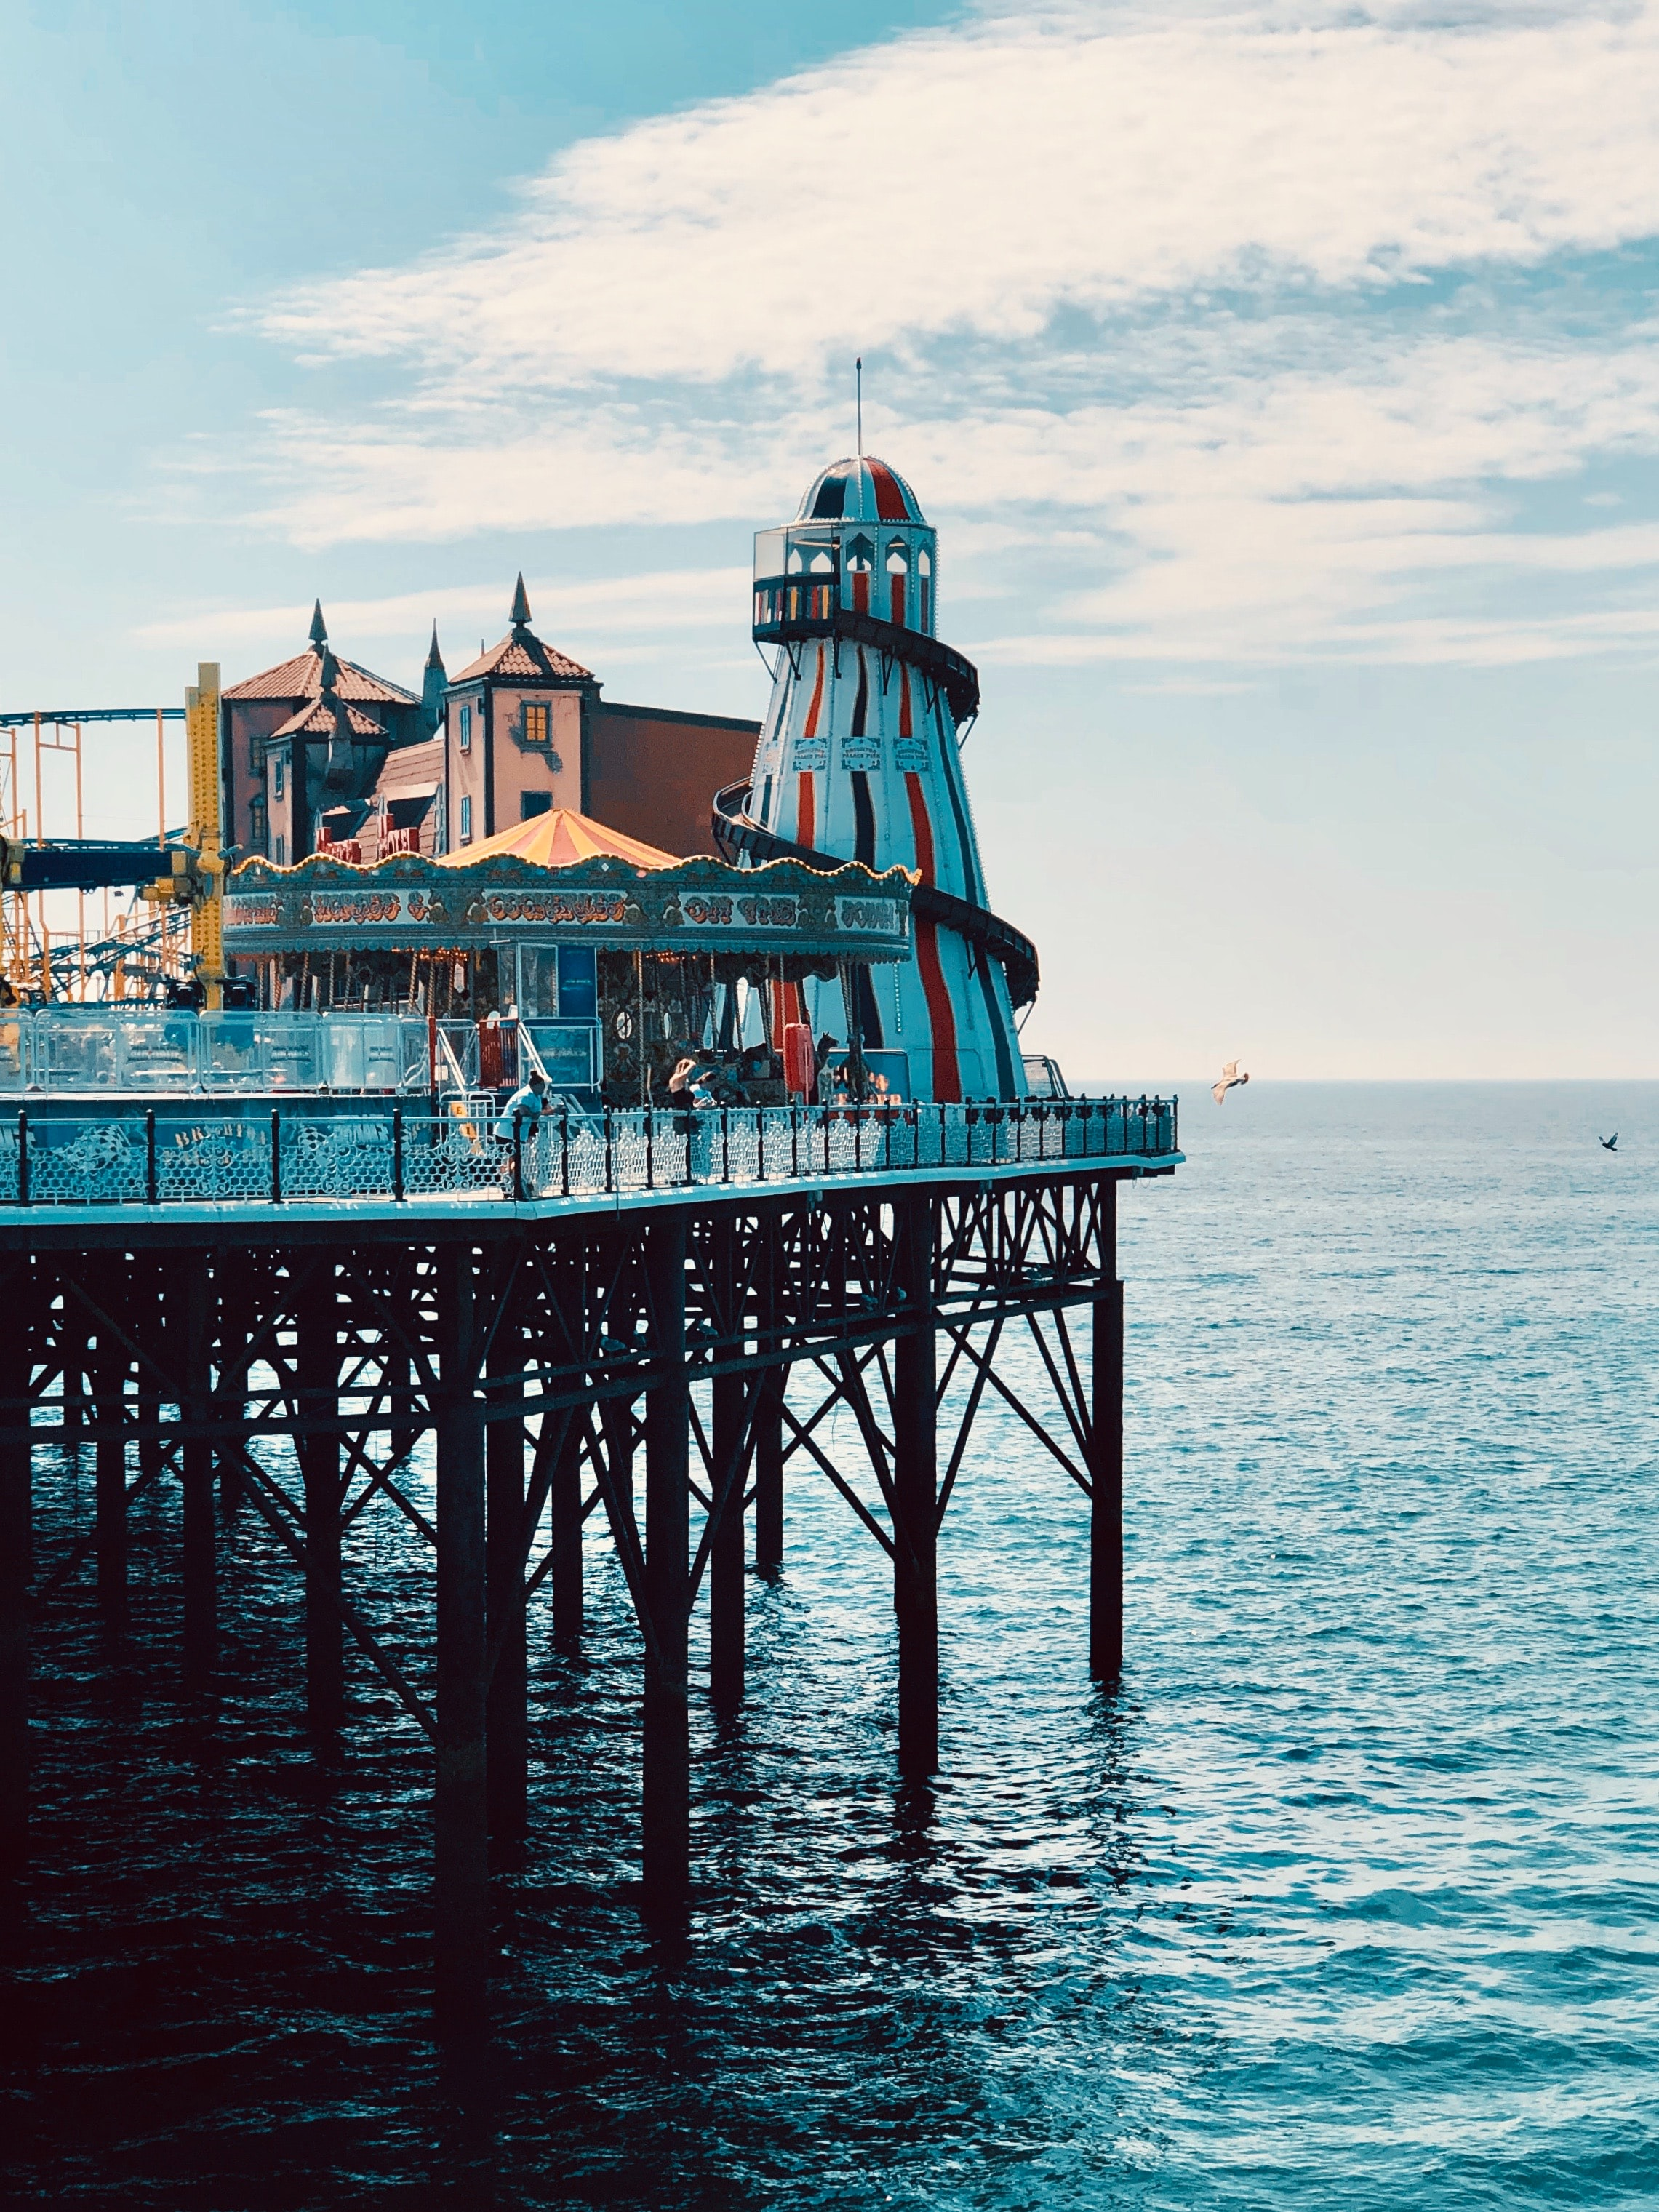
\includegraphics[width=6cm]{src/figures/brighton}}
    \videosupp{This is a description of a video supplement.}\label{videosupp:sv1}
    \figdata{This is a description of a data source.}\label{figdata:first}
    \figdata{This is another description of a data source.}\label{figdata:second}
    \figsrccode{This is a description of a source code.}\label{figsrccode:first}
\end{figure}

\subsection{Other Chemistry Niceties}

You can use commands from the \texttt{mhchem} and \texttt{siunitx} packages. For example: \ce{C32H64NO7S}; \SI{5}{\micro\metre}; \SI{30}{\degreeCelsius}; \SI{5e-17}{\Molar}

\subsection{Lists}

You can make lists with automatic numbering \dots

\begin{enumerate}
    \item Like this,
    \item and like this.
\end{enumerate}
\dots or bullet points \dots
\begin{itemize} 
    \item Like this,
    \item and like this.
\end{itemize}
\dots or with words and descriptions \dots
\begin{description}
    \item[Word] Definition
    \item[Concept] Explanation
    \item[Idea] Text
\end{description}

Some filler text, because empty templates look really poorly. \lipsum[1]